






\documentclass[a4paper]{article}

\usepackage{amsmath,amssymb,amsfonts}
\usepackage{graphicx,float,subfig}
\usepackage{booktabs}
\usepackage{fullpage}
\usepackage[colorlinks]{hyperref}
\usepackage{pdflscape}

\usepackage[font=small,labelfont=bf]{caption}

\renewcommand{\abstractname}{Aim}

\title{Estimation of Linear Attenuation Coefficient of Gamma Rays in Lead and Aluminum via Photoelectric and Compton Interaction}
\author{
    Oliver Kirkaptrick\footnote{s3725341@student.rmit.edu.au},
    Jackie Sholes\footnote{s3785864@student.rmit.edu.au},
    Anmolpreet Kaur Sodhi\footnote{s3838252@student.rmit.edu.au}
}


\begin{document}

\maketitle

\begin{abstract}
    The objective of this experiment is to determine the linear attenuation coefficient of gamma rays in lead and aluminum, and derive the mass absorption coefficient of these materials for gamma rays of varying energies. A gamma ray spectrometer is used to measure the decrease in the number of gamma rays detected as the thickness of a lead absorber is varied. The measurement of photoelectric or Compton interactions is used to calculate the attenuation coefficients. The spectrometer is calibrated using standard gamma-ray sources of known energies to ensure accurate measurement. The attenuation coefficients are then compared between the two materials, and the energy dependence of the coefficients is analyzed. The experimental results provide insights into the interaction of gamma rays with matter and have significant implications in a broad range of fields, such as radiation protection, nuclear medicine, and materials science.
\end{abstract}

\section{Relevant Theory}

As radiation passes through matter, some of that radiation will interact with the matter, giving the effect of reducing the total intensity of the radiation as it travels through the material. Similar to radioactive decay, we can model this reduction in intensity with an exponential relationship. Basically the exact same equation as well:

\begin{equation}
    I=I_{0}\mathrm{e}^{-\mu x}.
\end{equation}

Here, instead of decay rate $\gamma$ and time $t$, we have absorption coefficient $\mu$ and material thickness $x$. Similar to radioactive decay, where we have the concept of a half life, in attenuation of radiation by materials, we have the \textit{half value layer thickness}...which describes the thickness $x_{1/2}$ of material required such that $I=0.5I_{0}$. So, we let $I_{0}=1$ and thus $I=0.5$, and we can say

\begin{equation}
    I=I_{0}\mathrm{e}^{-\mu x}\Rightarrow 0.5 = \mathrm{e}^{-\mu x}\Rightarrow \frac{\ln{0.5}}{-\mu}=x_{1/2},
\end{equation}
or
\begin{equation}\label{eq:attenuation-coefficient}
    \mu=\frac{\ln{0.5}}{-x_{1/2}}.
\end{equation}
This half value layer thickness is then a convenient way to characterise materials with regards to their attenuation of radiation. If provided a half value layer thickness, we may then say for a given material which is $N$ ($\in\mathbb{R}^{+}$) times thicker than $x_{1/2}$, that the amount of attenuation is
\begin{equation}
    I=I_{0}\exp\left(-\mu\frac{N\ln0.5}{-\mu}\right)=I_{0}\exp\left(N\ln0.5\right)=I_{0}\frac{1}{2^{N}}.
\end{equation}
Another commonly quoted material property is the areal density of the material, which compensates for...material density. In all above equations, to get the areal density form, we replace $\mu$ with\footnote{sometimes high school algebra comes in handy}
\begin{equation}
    \frac{\mu}{\rho}\rho=\mu.
\end{equation}
An important property of a material which will affect its attenuation coefficient is the number of protons in the material. Materials with greater number of protons will tend to have higher attenuation coefficients due to their greater ability to interact with gamma rays via photoelectric, Compton, and pair production processes. This can be attributed to higher-Z materials providing more electrons to interact with the incoming gamma rays, leading to more scattering and absorption interactions, and thus faster attenuation.

Energy of incident gamma rays will also influence absorption coefficient. With increasing energy, gamma rays are more likely to pass through a given thickness of material without interacting. This will have the effect of requiring more material to accomplish equal attenuation, and thus reducing attenuation coefficient. Consider \eqref{eq:attenuation-coefficient}: as $x_{1/2}$ grows, it is clear that $\mu$ will become smaller---
\begin{equation}
    \mu\propto\frac{1}{x_{1/2}}.
\end{equation}
\section{Experiment Setup and Hardware}

The experiment utilized the following hardware, arranged as shown in~\autoref{fig:hardware-config}:
\begin{itemize}
\item NIM Bin and Power Supply
\item NaI(Tl) Crystal and Phototube Assembly
\item High Voltage Power Supply
\item Preamplifier
\item Amplifier
\item Oscilloscope
\item Ortec 928 Multi Channel Buffer, USB dual Port Memory cable, and PC with Maestro32 spectrum software for data analysis
\item $^{137}\mathrm{Cs}$, $^{22}\mathrm{Na}$, and $^{60}\mathrm{Co}$ gamma sources
\item Lead sheets of equal thickness, to be stacked together to create increasing attenuation.
\item Gain adjusted to xx to reach a maximum Oscilloscope reading of approximately 4 volts
\item Coarse gain set to xx, and fine gain set to 0.xx
\item Total gain set to xx
\end{itemize}

\begin{figure}[H]
\centering
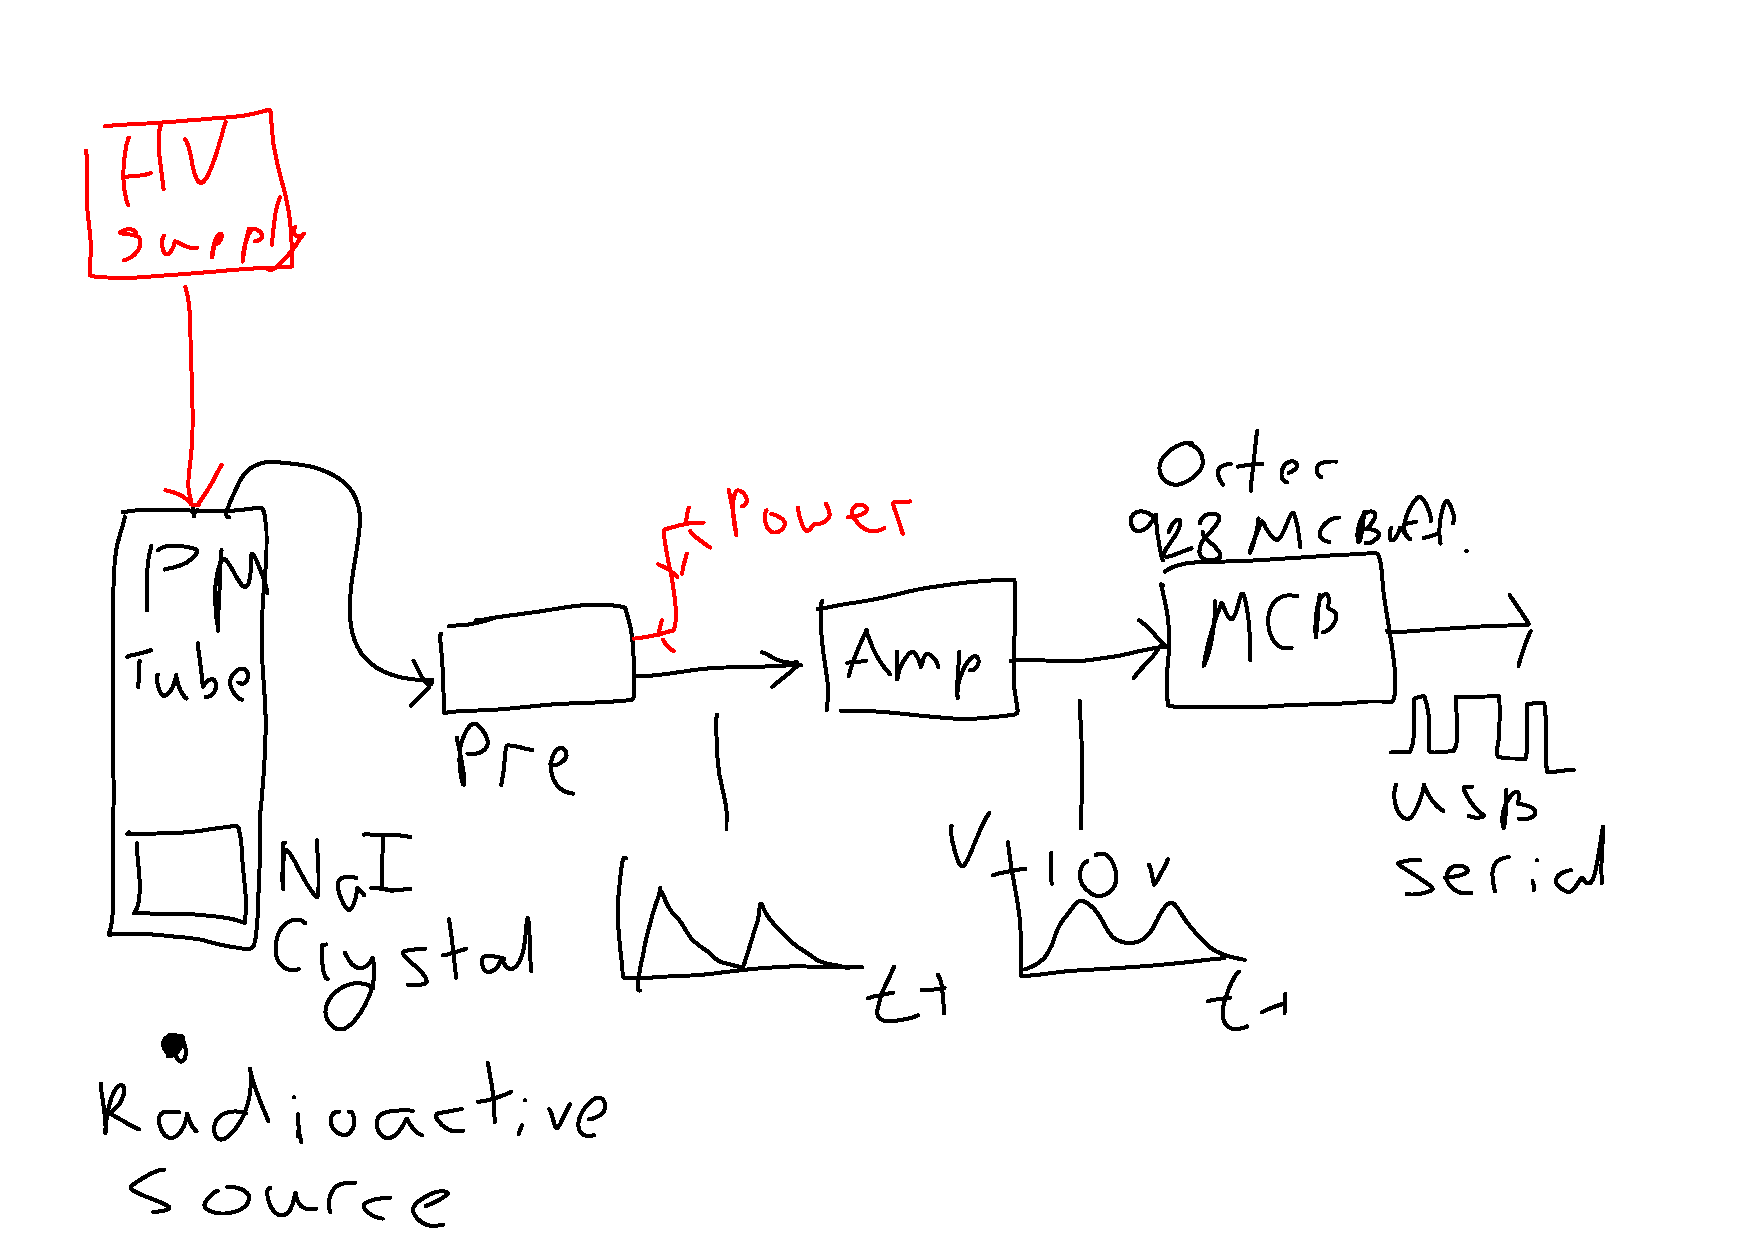
\includegraphics[width=0.6\textwidth]{figures/experiment-setup.pdf}
\caption{Base hardware configuration for calibration portion of the experiment--- $\pm$ Tube detects raw signals from a radioactive source placed approximately 2.5 cm away, which are then processed by the preamplifier and the amplifier. The signal peaks at around 10 V, and passes through the Multi-Channel Buffer for data analysis using Spectrum32 software on a computer.}
\label{fig:hardware-config}
\end{figure}
\subsection{Experimental Setup Procedures}

The setup procedures were carried out as follows:
\begin{enumerate}
\item Connect HV to the detector
\item Connect serial to preamp
\item Connect signal out of detector to 572A input
\item Connect T bridge out of uni to Oscilloscope and 928 MCB ADC in
\item Face of block set 4 cm away from face of detector
\item Set initial scale from Oscilloscope to 500 mV
\item Set initial pulse width to 3.36 $\mu$s
\end{enumerate}
\section{Calibration Using $^{137}\mathrm{Cs}$, $^{22}\mathbf{Na}$, and $^{60}\mathrm{Co}$}
\subsection{Calibration}
\begin{itemize}
    \item initial height of photopeak was 968 counts at live value of 20.58 seconds
    \item integration time decreased to 5
    \item 5 seconds produced 267 counts, total gross area of ROI was 13576 counts
    \item ROI was set on 660.21 keV peak, and calibrated to 662
    \item 662 keV peak was identified as 662 keV, at bin 767.53, with FWHM of 36.31m library identified as cs 137
\end{itemize}

\subsection{Spectrum of $^{137}$Cs}
\begin{figure}[H]
    \centering
    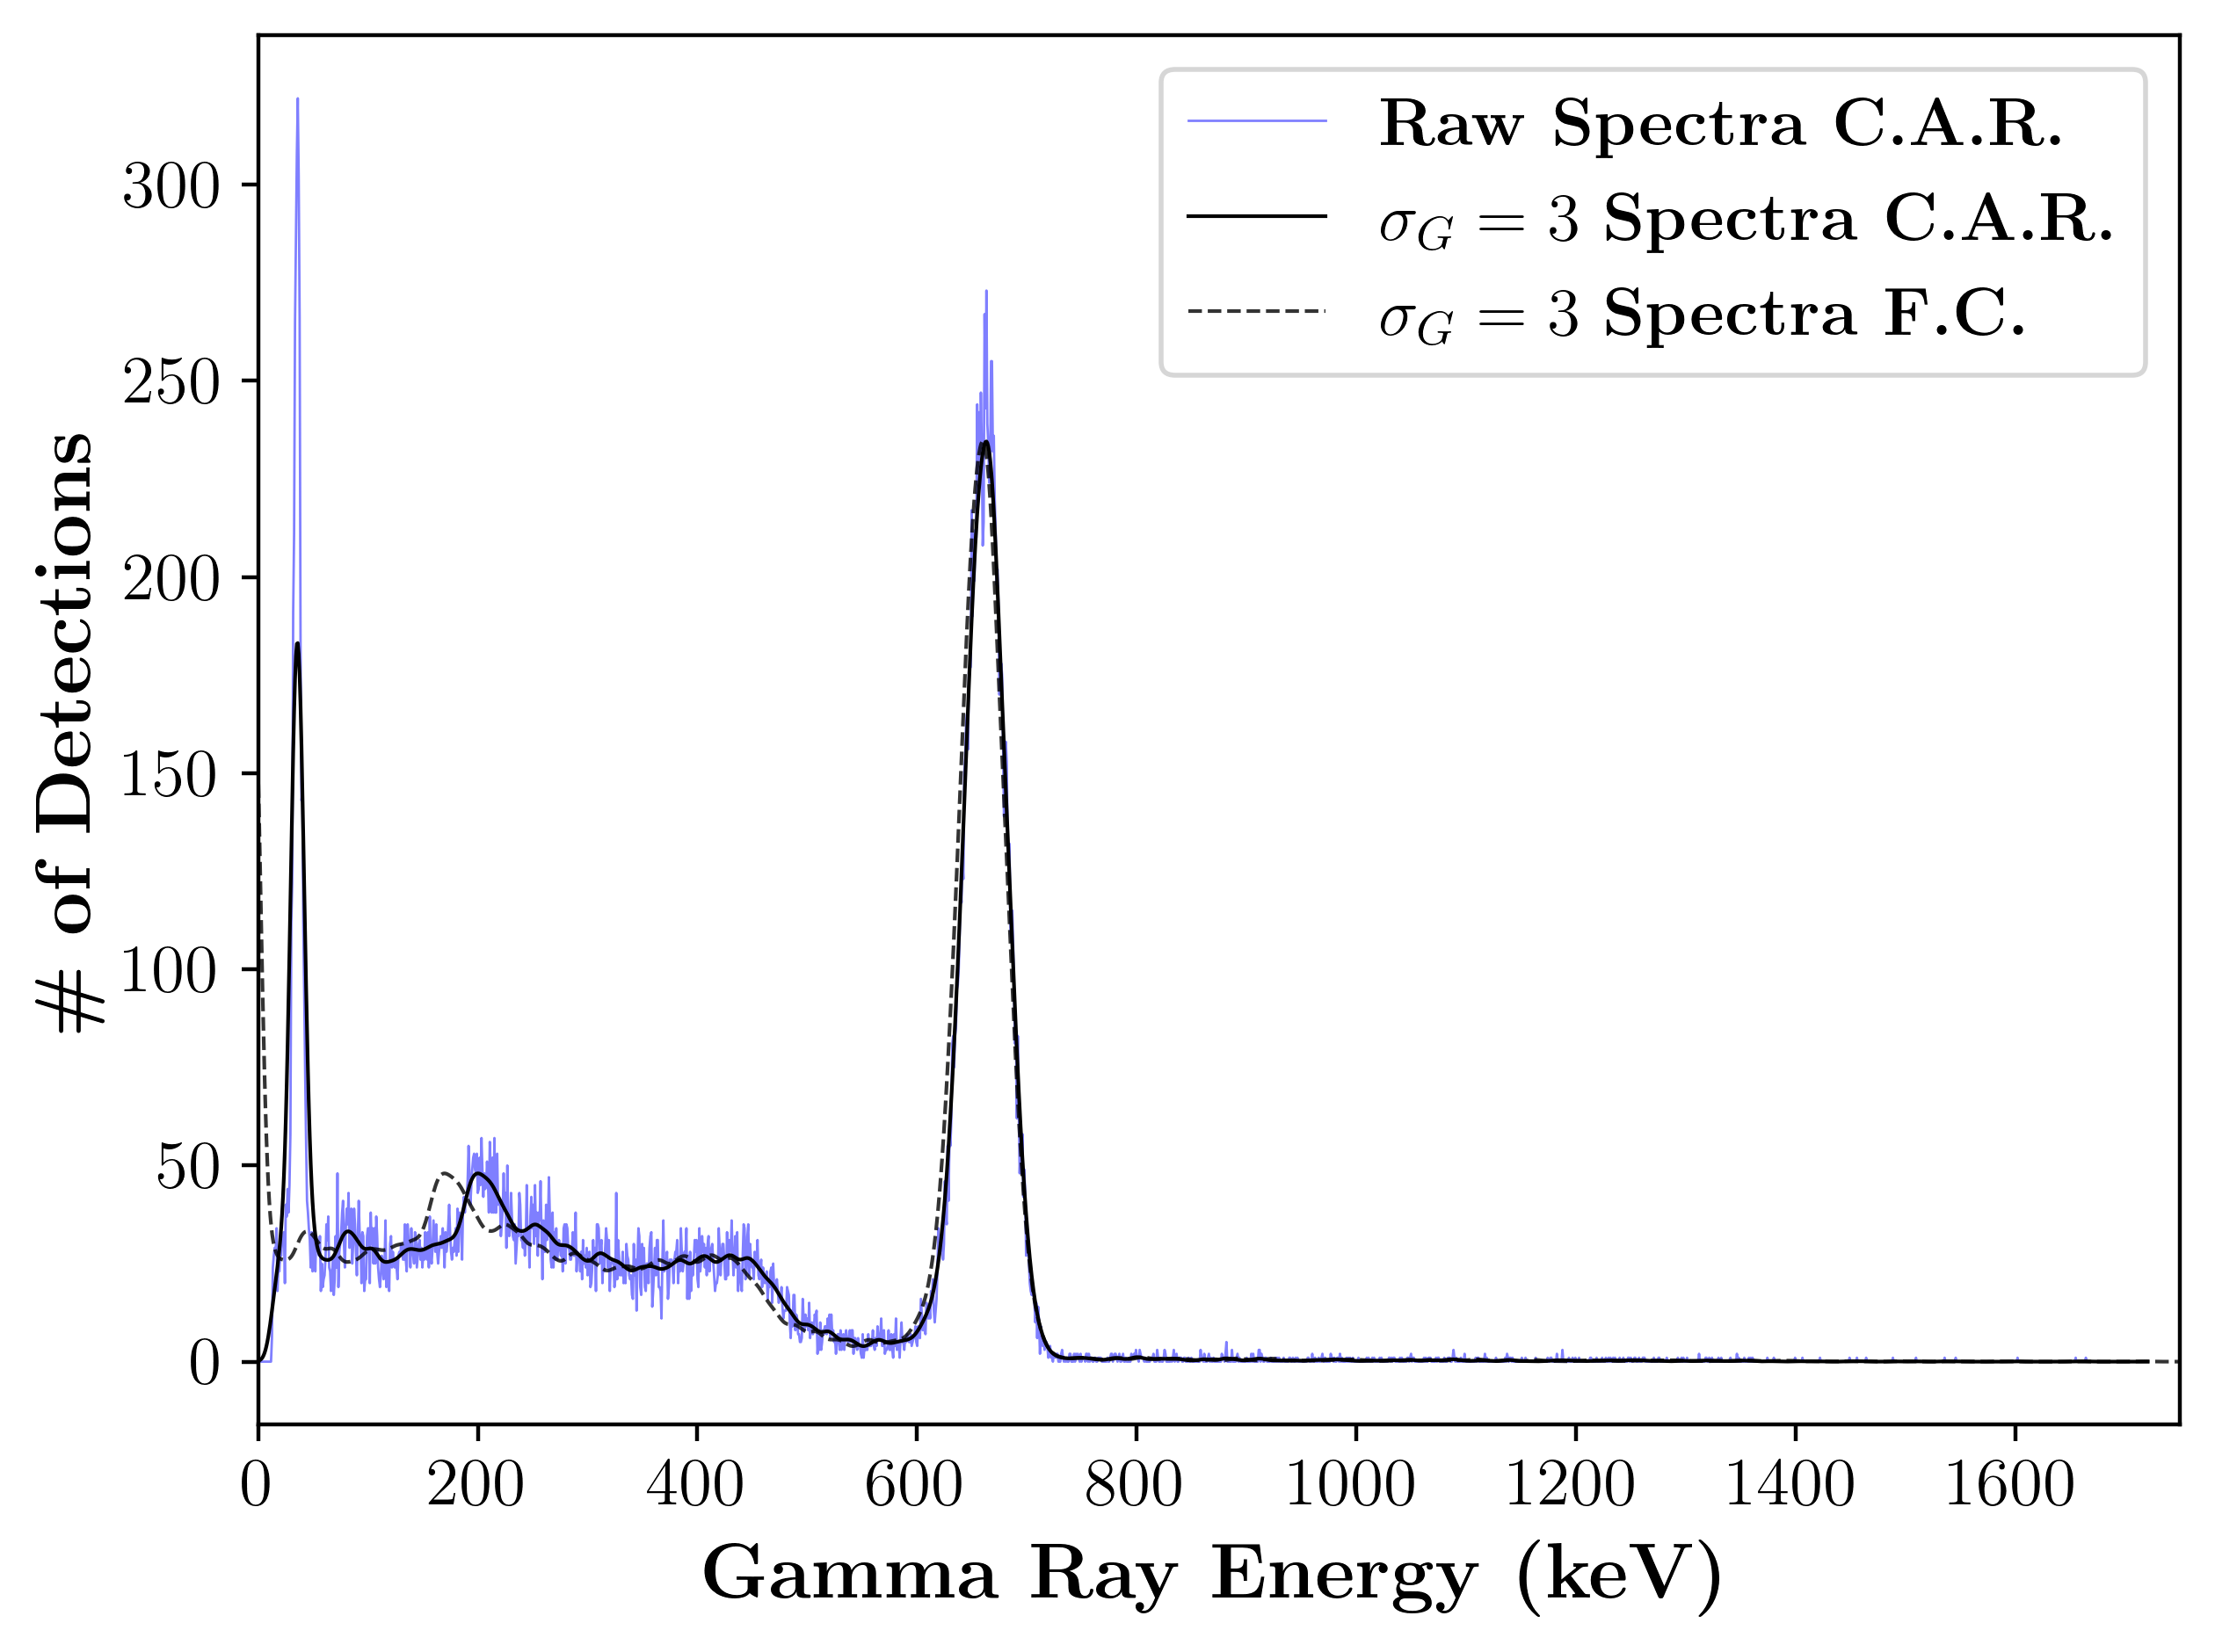
\includegraphics[width=0.75\textwidth]{figures/calibration_spectrum_cs_counts_overlay_both_mca.png}
    \caption{$^{137}$Cs pectra of counts associated with varying energy bins. Two distinct peaks were identified, with peaks described in body text}
\end{figure}
\begin{itemize}
    \item again, cesium was 4 cm away from face of detector
    \item 32 keV peak was identified as 32.01 keV, at bin 42.31, with FWHM as 7.21
    % \item \verb|$MCA_CAL:-4.452449E+000 8.674188E-001 0.000000E+000 keV|
    \item \textbf{Data saved at: ./data/calibration\_spectrum\_cs.*}
\end{itemize}

\subsection{Spectrum of $^{22}$Na}
\begin{figure}[H]
    \centering
    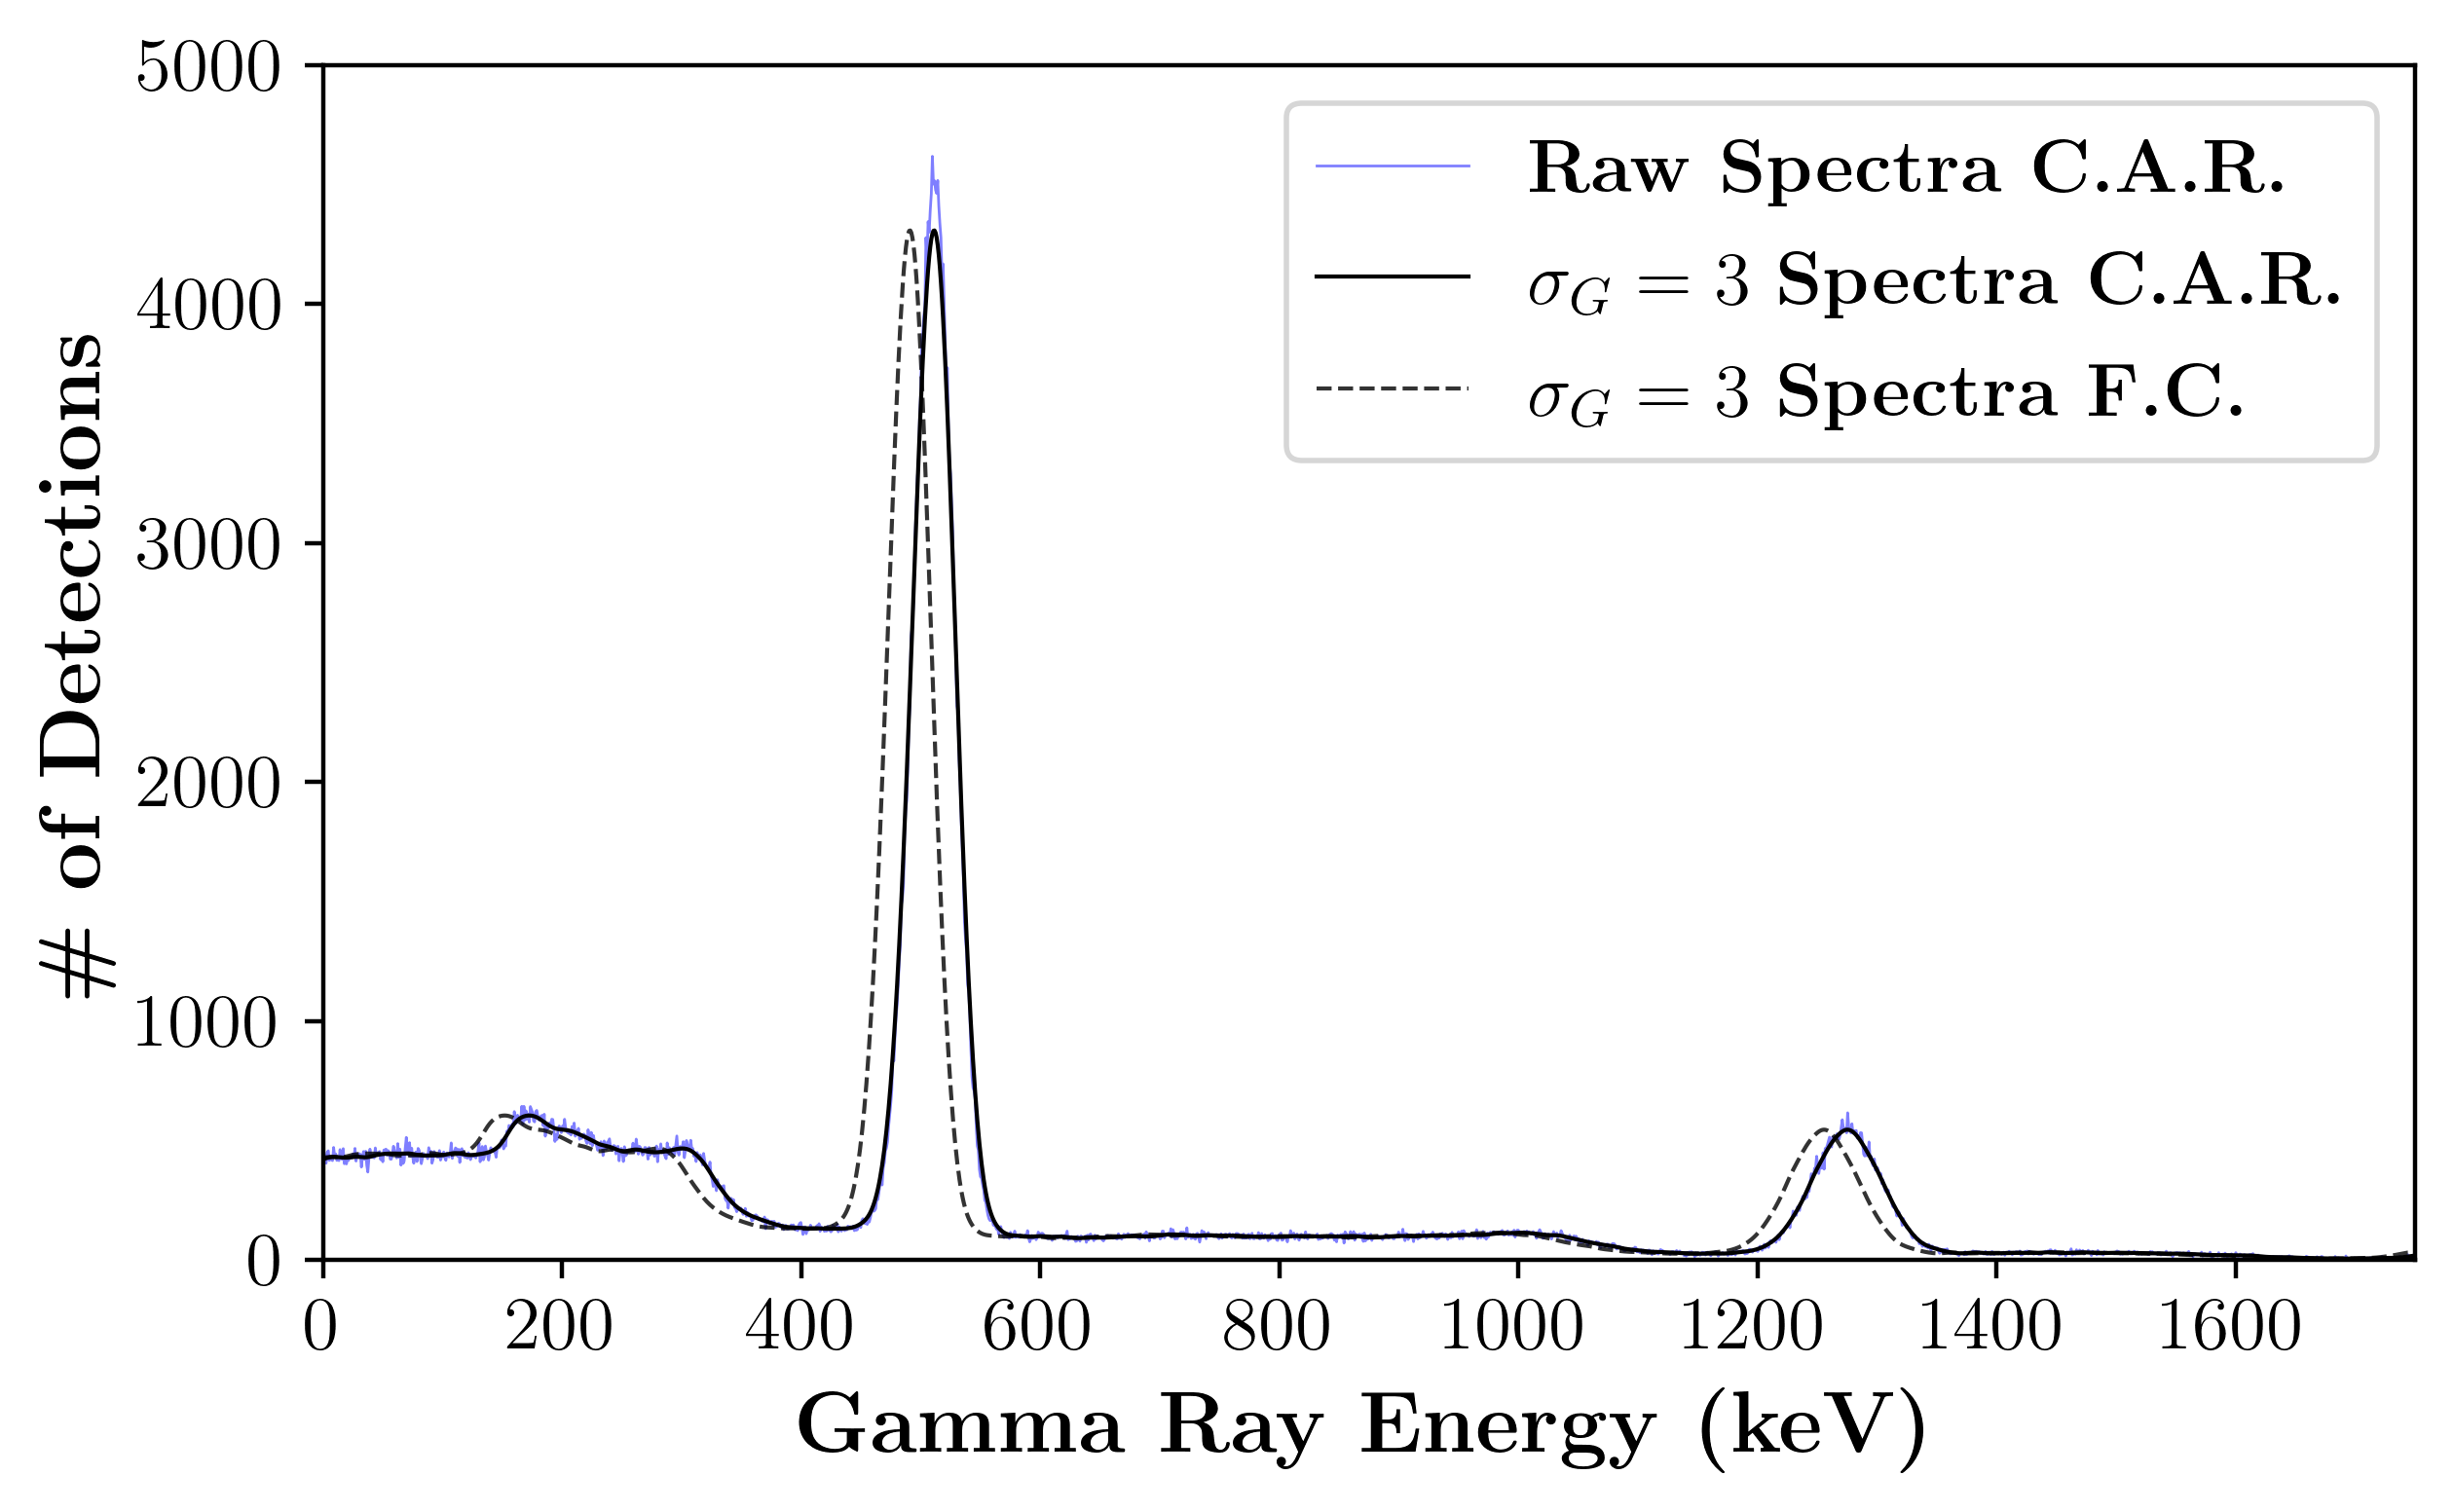
\includegraphics[width=0.75\textwidth]{figures/calibration_spectrum_na_counts_overlay_both_mca.png}
    \caption{$^{22}$Na spectra of counts associated with varying energy bins. Two distinct peaks were identified, with peak details outlined in body text.}
\end{figure}
\begin{itemize}
    \item again, sodium was place 4 cm away from face of detector, however, offset to the left this time
    \item first uncalibrated peak at 516.62 keV, bin at 614.58, should be 511 keV, FWHM was 38.55,suggested cesium
    \item second uncalibrated peak at 1246.74 keV, at bin 1483.15, should be 1275, FWHM was 58.54
    \item calibration used 511 peak
    \item after calibration first peak is at 511 keV, FWHM is 40.21, at bin 614.60, library suggests ytrium 88
    \item after calibration second peak is at 1274.98 keV, at bin 1483.12, FWHM was 61.69, library suggests sodium Na-22
    % \item \verb|-2.948798E+001 8.943686E-001 0.000000E+000 keV|
    \item \textbf{Data saved at: ./data/calibration\_spectrum\_na.*}
\end{itemize}

\subsection{Spectrum of $^{60}$Co}
\begin{figure}[H]
    \centering
    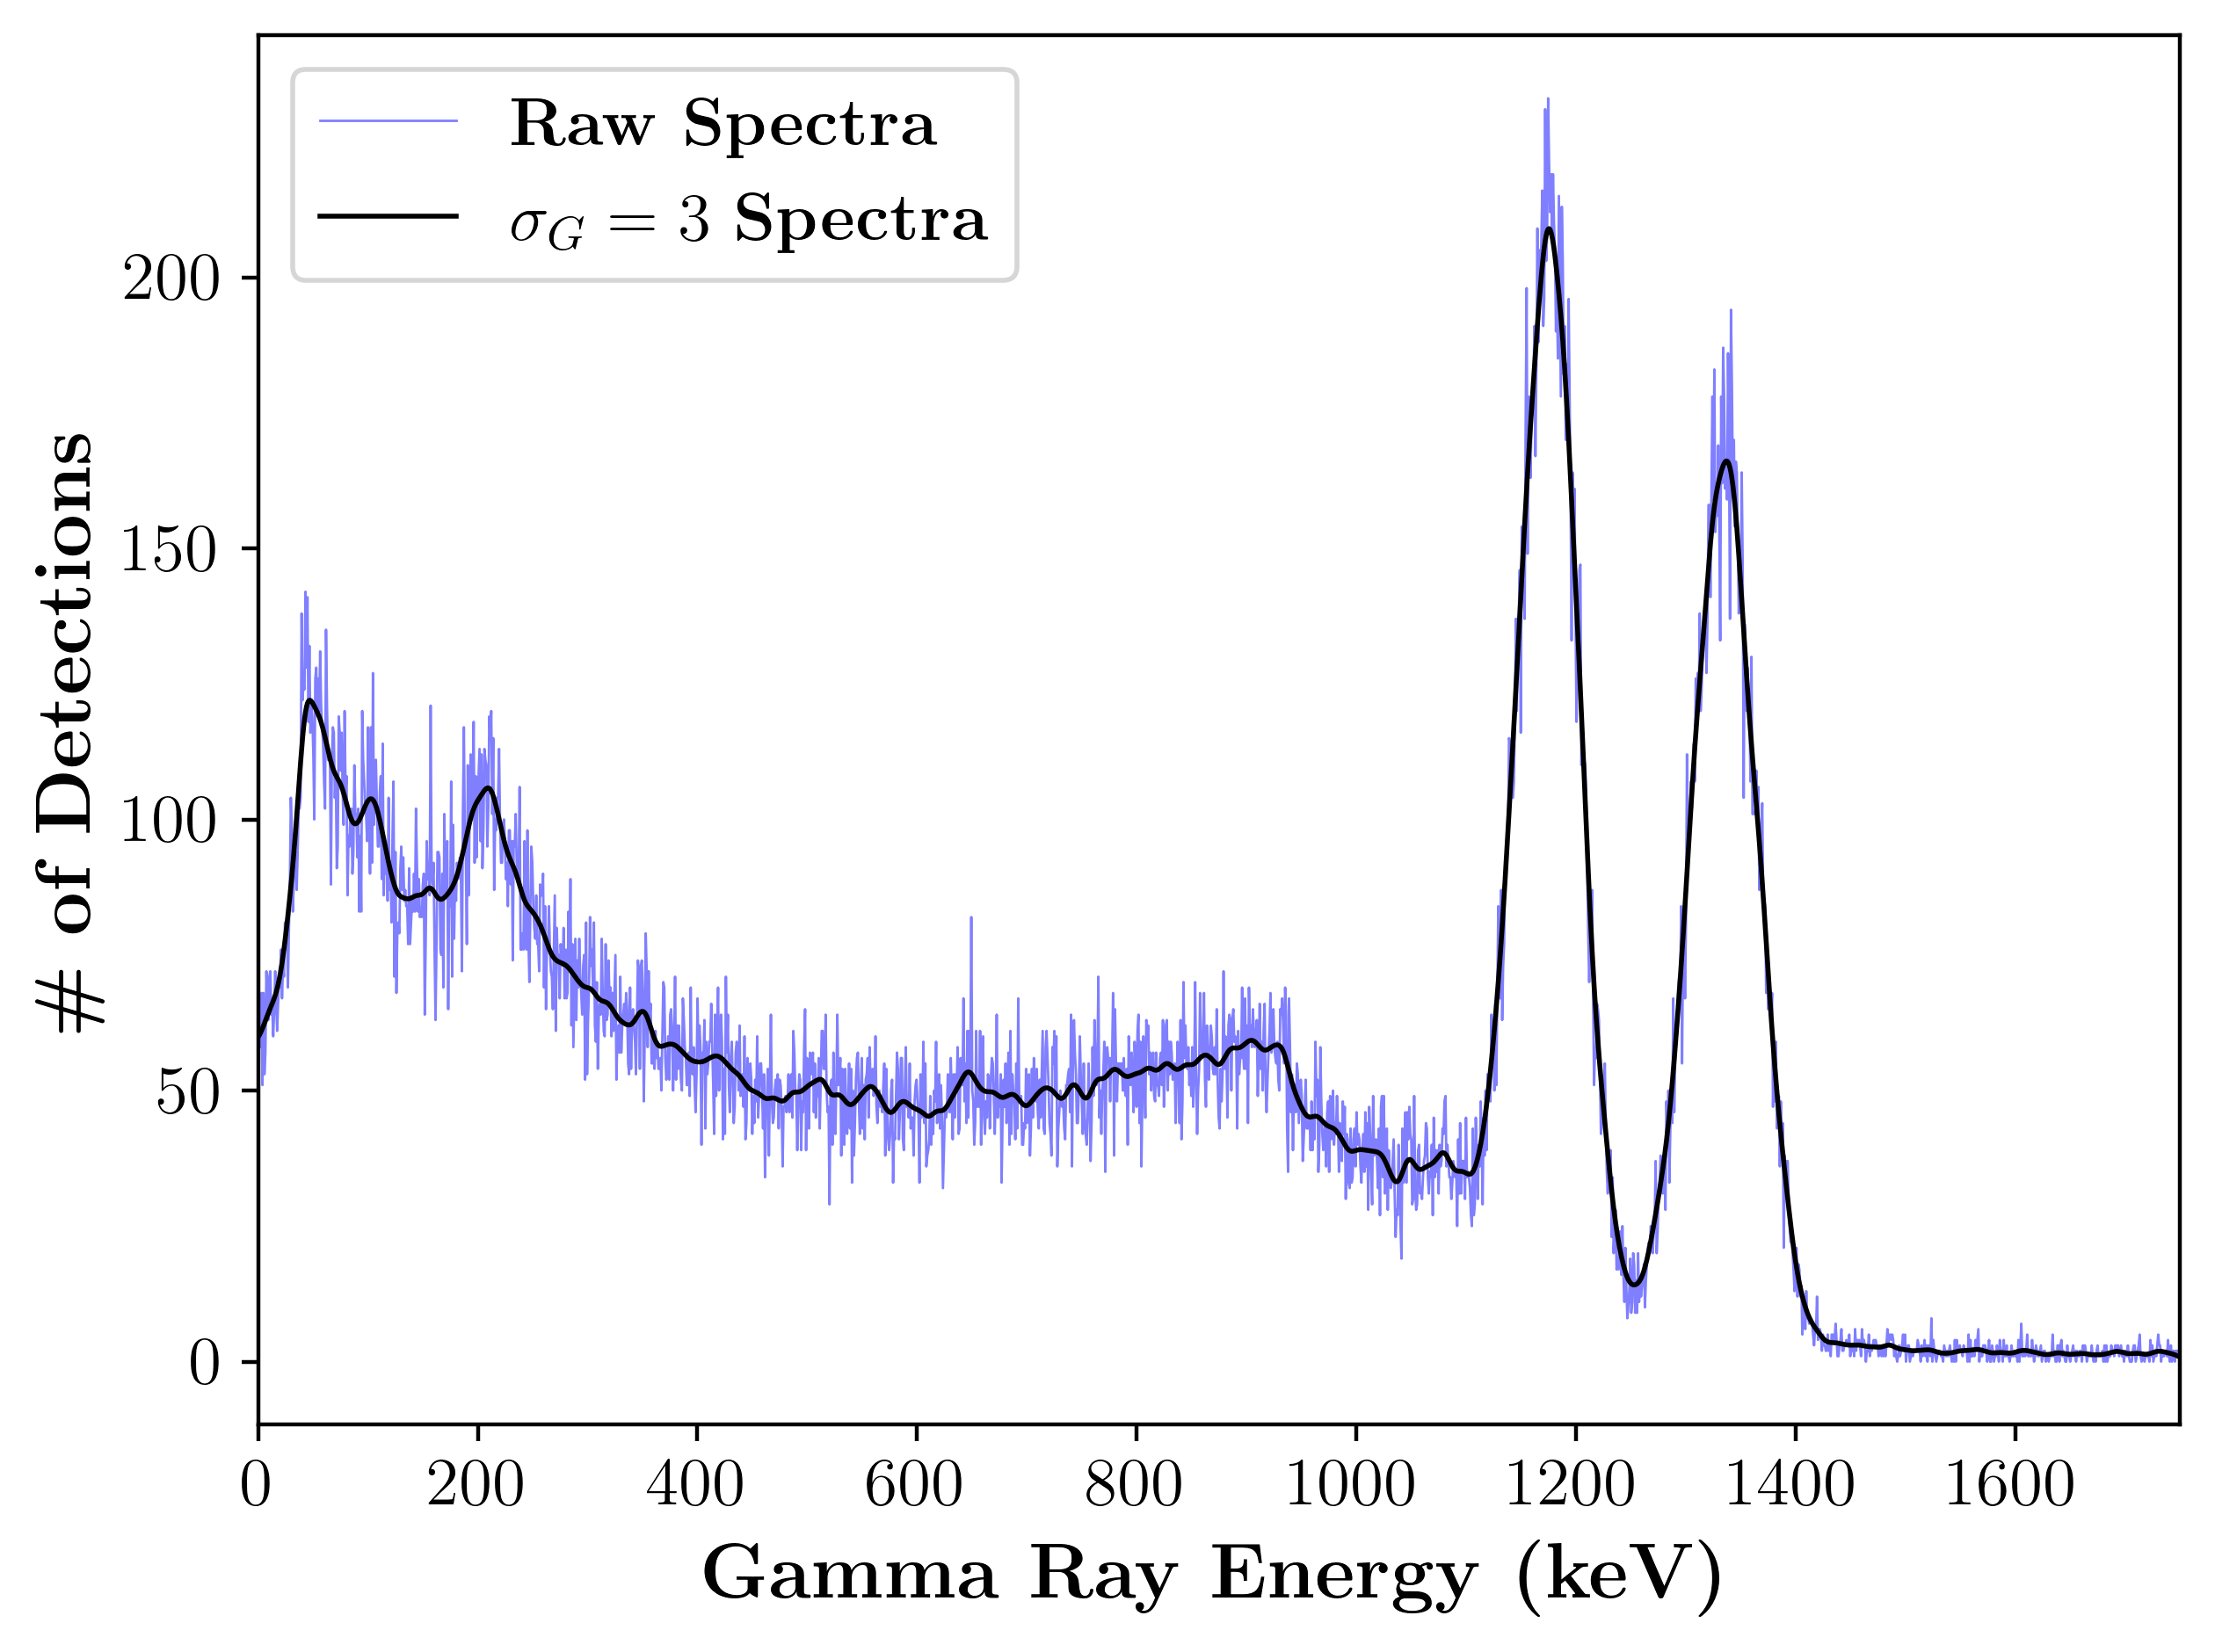
\includegraphics[width=0.75\textwidth]{figures/calibration_spectrum_co_counts_overlay_final_mca.png}
    \caption{$^{60}$Co spectra of counts associated with varying energy bins. Two distinct peaks were identified, with centerpoints described in body.}
\end{figure}
\begin{itemize}
    \item recorded for 100 seconds
    \item again, cobalt was placed 4 cm away from face of detector
    \item reading on Oscilloscope was noticably higher than that of cesium and sodium
    \item size of peaks and number of counts on Maestro32 were significantly lower than those of cesium and sodium
    \item two peaks were identified, neighbouring one another
    \item first uncalibrated peak was at 1170.52 keV, at bin 1364.37, FWHM was 55.39
    \item second uncalibrated peak was at 1329.53 keV, bin was 1545.13, FWHM was 55.97
    \item first photo peak calibrated to 1173.2 keV (did nothing), second to 1332.5 keV
    \item first peak calibrated to 1173.02 keV, bin at 1366.44, FWHM was 51.17, library suggested cobalt 60
    \item second peak calibrated to 1333, at bin 1544.74, FWHM was 57.28, library suggested cobalt 60
    \item after calibration, first peak calibrated to 1172.95 at bin 1364.97, FWHM was 56.38
    % \item \verb|-5.031831E+001 8.952744E-001 0.000000E+000 keV|
    \item \textbf{Data saved at: ./data/calibration\_spectrum\_co.*}
\end{itemize}

\subsection{Background}
\begin{figure}[H]
    \centering
    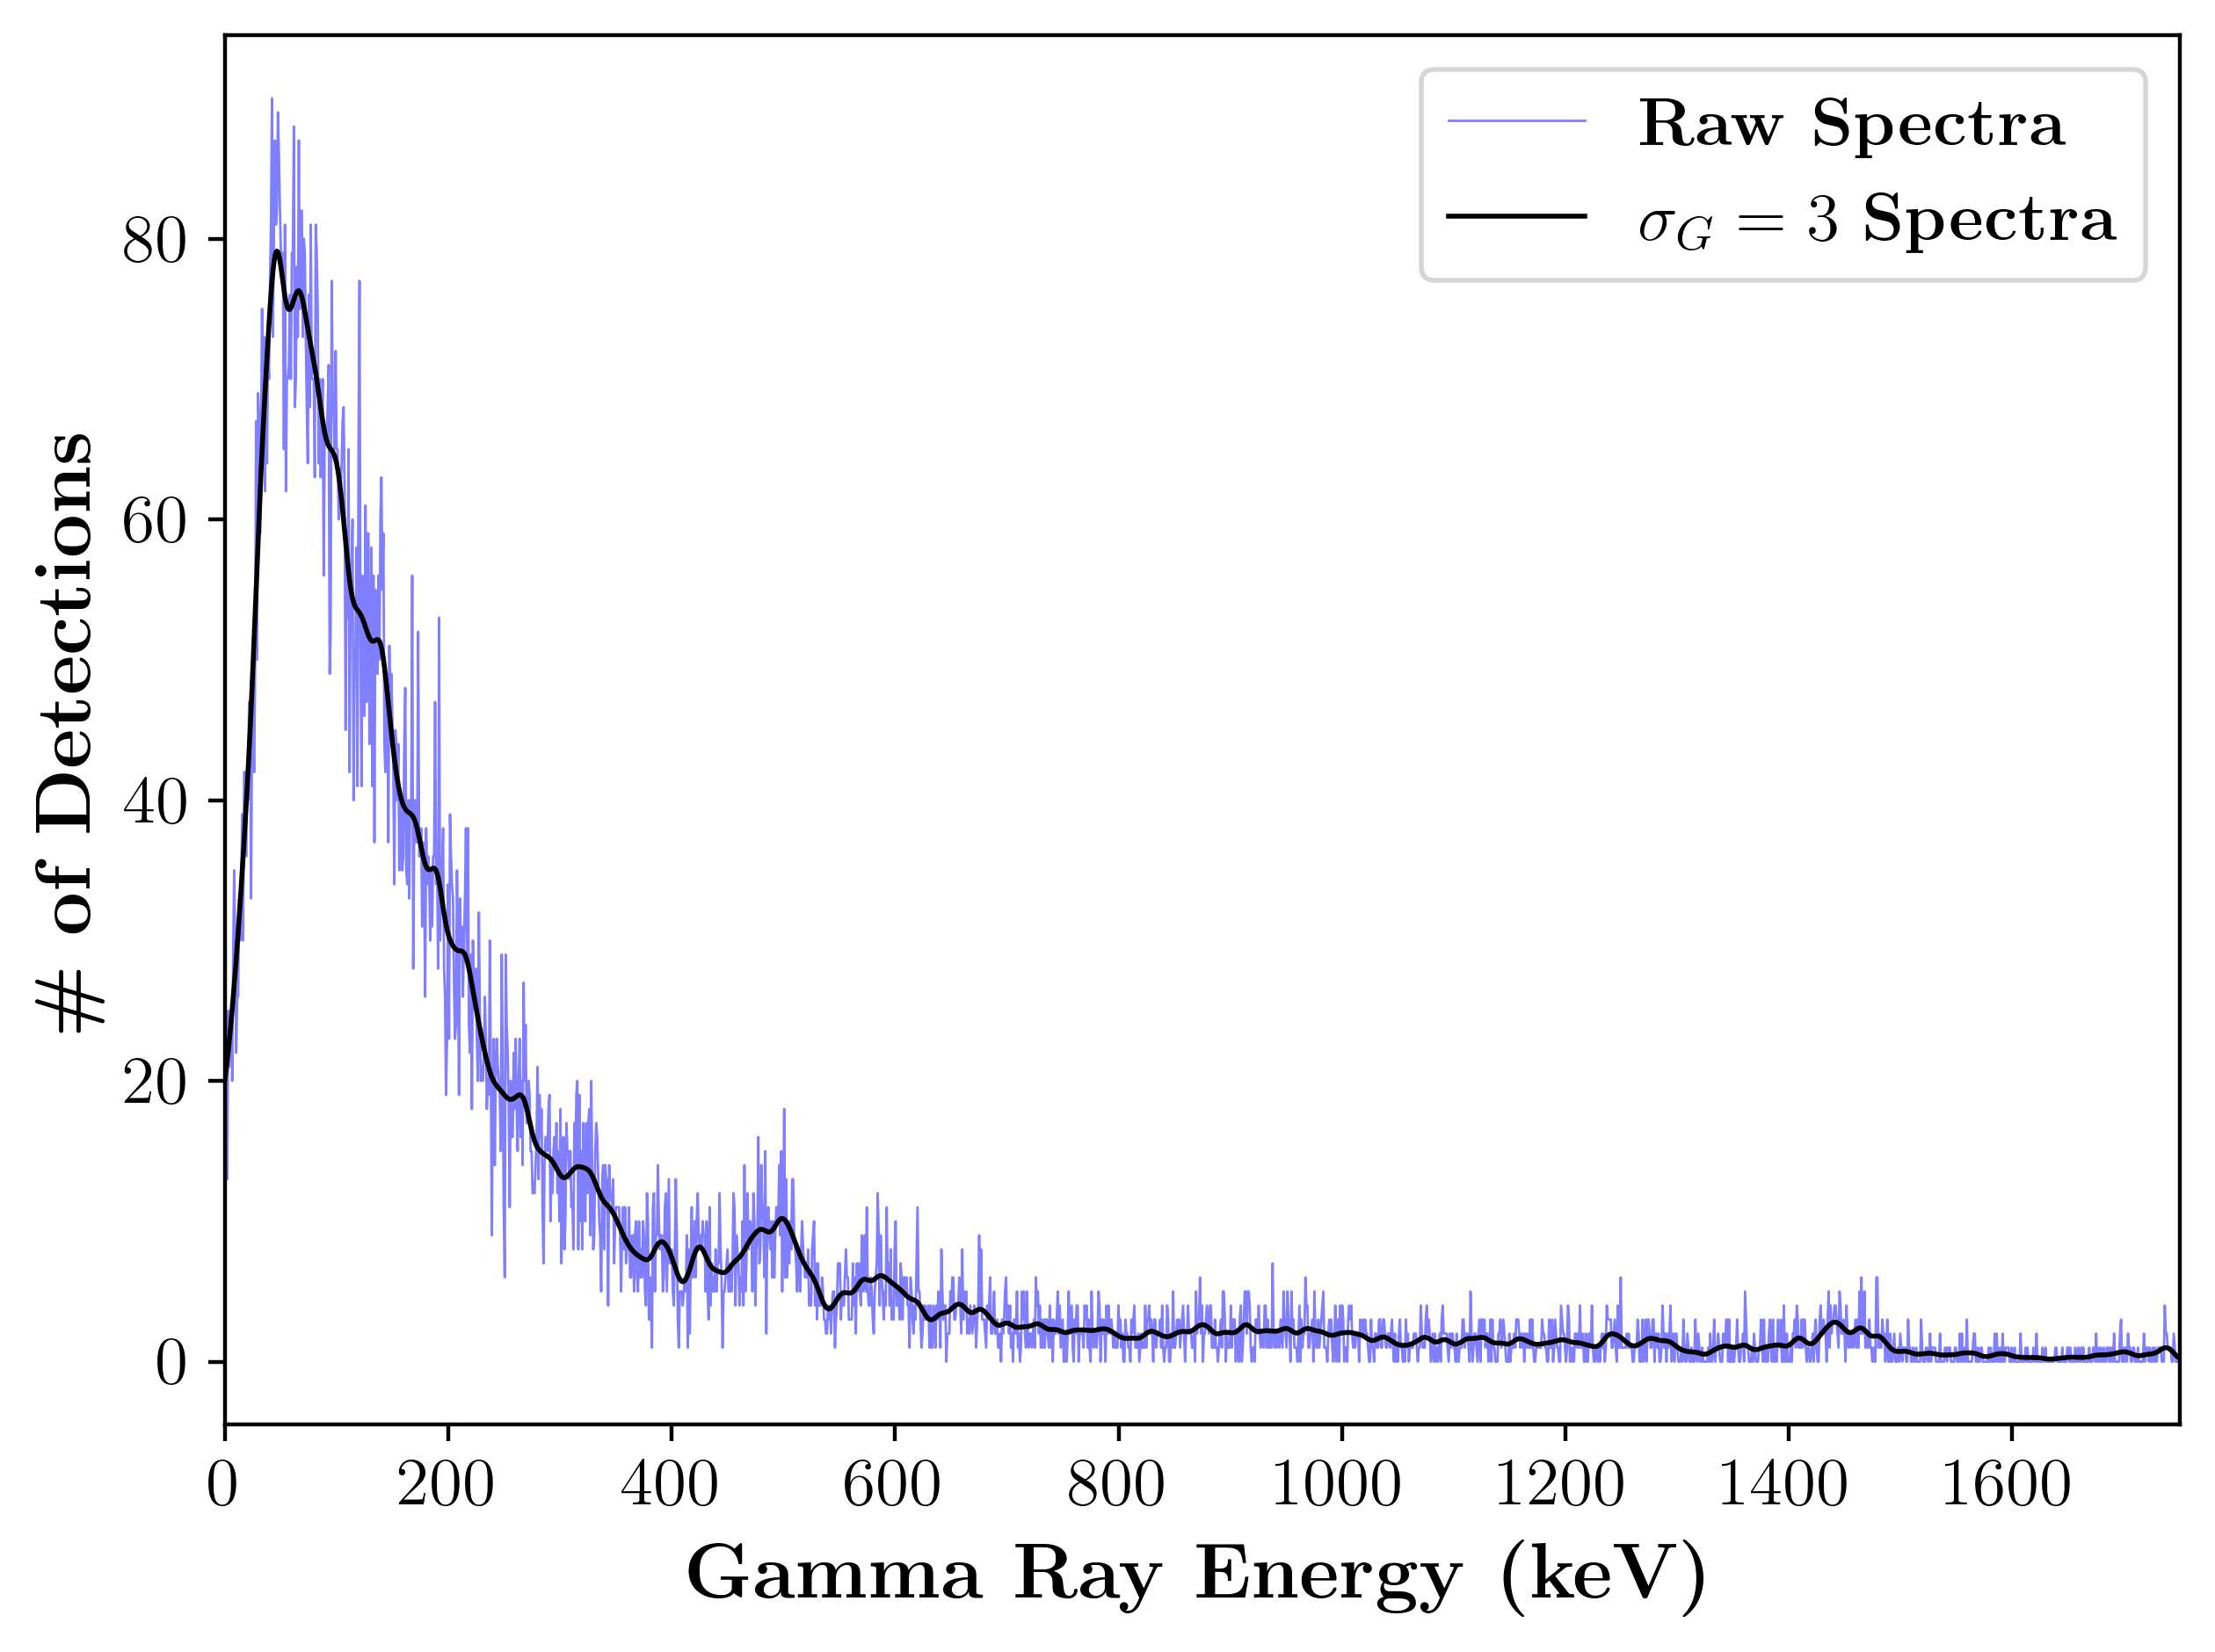
\includegraphics[width=0.75\textwidth]{figures/background_counts_overlay.png}
    \caption{Background counts spectra.}
\end{figure}
\begin{itemize}
    \item with no sample, a background spectrum was recorded
    \item peak was 153.73 keV, FWHM was 1.04
    \item library suggested Xenon 138
    \item \textbf{Data saved at: ./data/calibration\_spectrum\_bg.*}
\end{itemize}

\section{Lead Plate Measurement}
\begin{itemize}
    \item lead plates were measured at each corner
\end{itemize}
\begin{table}[H]
    \centering
    \caption{Thicknesses of lead attenuators, measured at corners. Average value will be taken when trying to calculate HVL.}
    \begin{tabular}{c c c c c}
        \toprule
        \textbf{Plate No.} & \textbf{Meas. 1} & \textbf{Meas. 2} & \textbf{Meas. 3} & \textbf{Meas. 4}\\
        \midrule
        1 & 1.82 mm & 1.94 mm & 1.91 mm & 1.79 mm\\
        2 & 1.75 mm & 1.93 mm & 1.97 mm & 1.65 mm\\
        3 & 1.83 mm & 1.93 mm & 1.88 mm & 1.73 mm\\
        4 & 1.83 mm & 1.68 mm & 1.79 mm & 1.95 mm\\
        5 & 1.66 mm & 1.89 mm & 1.83 mm & 1.86 mm\\
        6 & 1.88 mm & 1.86 mm & 1.81 mm & 1.83 mm\\
        7 & 1.61 mm & 1.89 mm & 1.84 mm & 1.88 mm\\
        8 & 1.86 mm & 1.94 mm & 1.91 mm & 2.06 mm\\
        9 & 1.84 mm & 1.84 mm & 1.77 mm & 1.84 mm\\
        10 & 1.86 mm & 1.77 mm & 1.93 mm & 1.89 mm\\
        \bottomrule
    \end{tabular}
\end{table}

\section{Aluminum Plate Measurement}

\begin{table}[H]
    \centering
    \caption{Thicknesses of Aluminum attenuator, at corners.}
    \begin{tabular}{c c c c c}
        \toprule
        \textbf{Plate No.} & \textbf{Meas. 1} & \textbf{Meas. 2} & \textbf{Meas. 3} & \textbf{Meas. 4}\\
        \midrule
        1 & 6.31 mm & 6.31 mm & 6.31 mm & 6.31 mm\\
        \bottomrule
    \end{tabular}
\end{table}

\section{Attenuation Coefficient Estimation}

\begin{figure}[H]
    \centering
    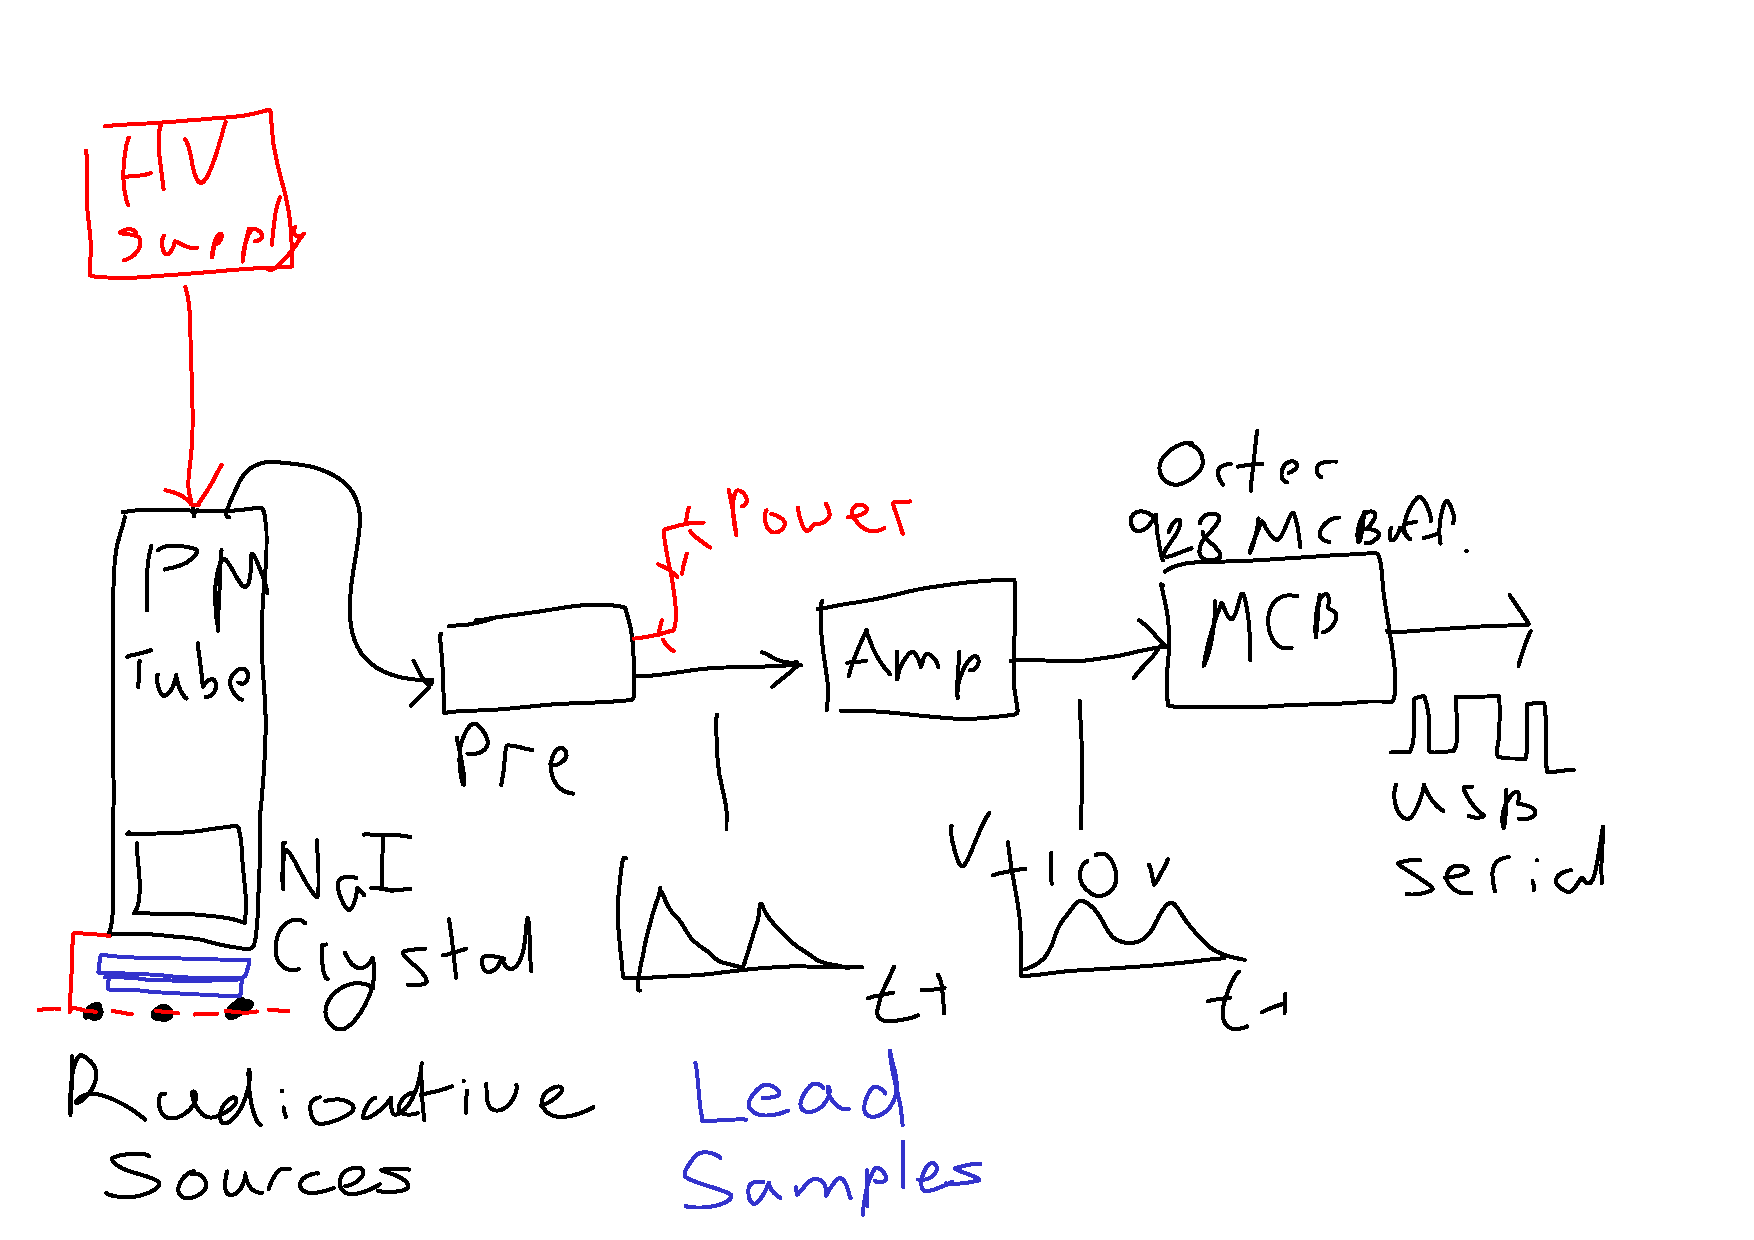
\includegraphics[width=0.75\textwidth]{figures/attenuation-setup.pdf}
    \caption{Modification of experiment setup to compare detections with increasing amounts of attenuating material (lead).}
\end{figure}

\begin{itemize}
    \item all samples placed in front of detector
    \item went sodium, cesium, cobalt
\end{itemize}
\subsection{Recording 1, no shielding, $N_{P}=0$}
\begin{itemize}
    \item file saved at \verb|attenuator_0.*|
    \item cobalt 1333 peak overlaps with sodium 1274 peak
    \item recording for live time of 60s
    \item we'll use the sodium 511 and cobalt 1274 keV peaks
    \item sodium cesium 662 keV peak had net area of 160608 $\pm$ 732 net area
    \item cobalt 1274 keV peak had net area of 11409 $\pm$ 353 net area
\end{itemize}
\subsection{Recording 2, $N_{P}=1$}
\begin{itemize}
    \item file saved at \verb|attenuator_1.*|
    \item lead sheet 1 placed directly against detector face
    \item recording for live time of 60s
    \item cesium 662 keV peak had net area of 129426 $\pm$ 697
    \item cobalt 1333 keV peak had net area of 10218 $\pm$ 273
\end{itemize}

\subsection{Recording 3, $N_{P}=2$}
\begin{itemize}
    \item file saved at \verb|attenuator_2.*|
    \item lead sheet 2 placed directly against detector face
    \item recording for live time of 60s
    \item cesium 662 keV peak had net area of 102890 $\pm$ 696
    \item cobalt 1333 keV peak had net area of 8794 $\pm$ 278
\end{itemize}

\subsection{Recording 4, $N_{P}=3$}
\begin{itemize}
    \item file saved at \verb|attenuator_3.*|
    \item lead sheet 3 placed directly against detector face
    \item recording for live time of 60s
    \item cesium 662 keV peak had net area of 81614 $\pm$ 653
    \item cobalt 1333 keV peak had net area of 7794 $\pm$ 259
\end{itemize}

\subsection{Recording 5, $N_{P}=4$}
\begin{itemize}
    \item file saved at \verb|attenuator_4.*|
    \item lead sheet 4 placed directly against detector face
    \item recording for live time of 60s
    \item cesium 662 keV peak had net area of 65960 $\pm$ 626
    \item cobalt 1333 keV peak had net area of 6595 $\pm$ 259
\end{itemize}

\subsection{Recording 6, $N_{P}=5$}
\begin{itemize}
    \item file saved at \verb|attenuator_5.*|
    \item lead sheet 5 placed directly against detector face
    \item recording for live time of 60s
    \item cesium 662 keV peak had net area of 52527 $\pm$ 585
    \item cobalt 1333 keV peak had net area of 6112 $\pm$ 229
\end{itemize}

\subsection{Recording 7, $N_{P}=6$}
\begin{itemize}
    \item file saved at \verb|attenuator_6.*|
    \item lead sheet 6 placed directly against detector face
    \item recording for live time of 60s
    \item cesium 662 keV peak had net area of 41935 $\pm$ 537
    \item cobalt 1333 keV peak had net area of 5520 $\pm$ 204
\end{itemize}

\subsection{Recording 8, $N_{P}=7$}
\begin{itemize}
    \item file saved at \verb|attenuator_7.*|
    \item lead sheet 7 placed directly against detector face
    \item recording for live time of 60s
    \item cesium 662 keV peak had net area of 32744 $\pm$ 542
    \item cobalt 1333 keV peak had net area of 4196 $\pm$ 248
\end{itemize}

\subsection{Recording 9, $N_{P}=8$}
\begin{itemize}
    \item file saved at \verb|attenuator_8.*|
    \item lead sheet 8 placed directly against detector face
    \item recording for live time of 60s
    \item cesium 662 keV peak had net area of 27384 $\pm$ 491
    \item cobalt 1333 keV peak had net area of 3713 $\pm$ 237
\end{itemize}

\subsection{Recording 10, $N_{P}=9$}
\begin{itemize}
    \item file saved at \verb|attenuator_9.*|
    \item lead sheet 9 placed directly against detector face
    \item recording for live time of 60s
    \item cesium 662 keV peak had net area of 22346 $\pm$ 471
    \item cobalt 1333 keV peak had net area of 3983 $\pm$ 174
\end{itemize}

\subsection{Recording 11, $N_{P}=10$}
\begin{itemize}
    \item file saved at \verb|attenuator_10.*|
    \item lead sheet 10 placed directly against detector face
    \item recording for live time of 60s
    \item cesium 662 keV peak had net area of 17062 $\pm$ 447
    \item cobalt 1333 keV peak had net area of 3004 $\pm$ 1203
\end{itemize}

\begin{figure}[H]
    \centering
    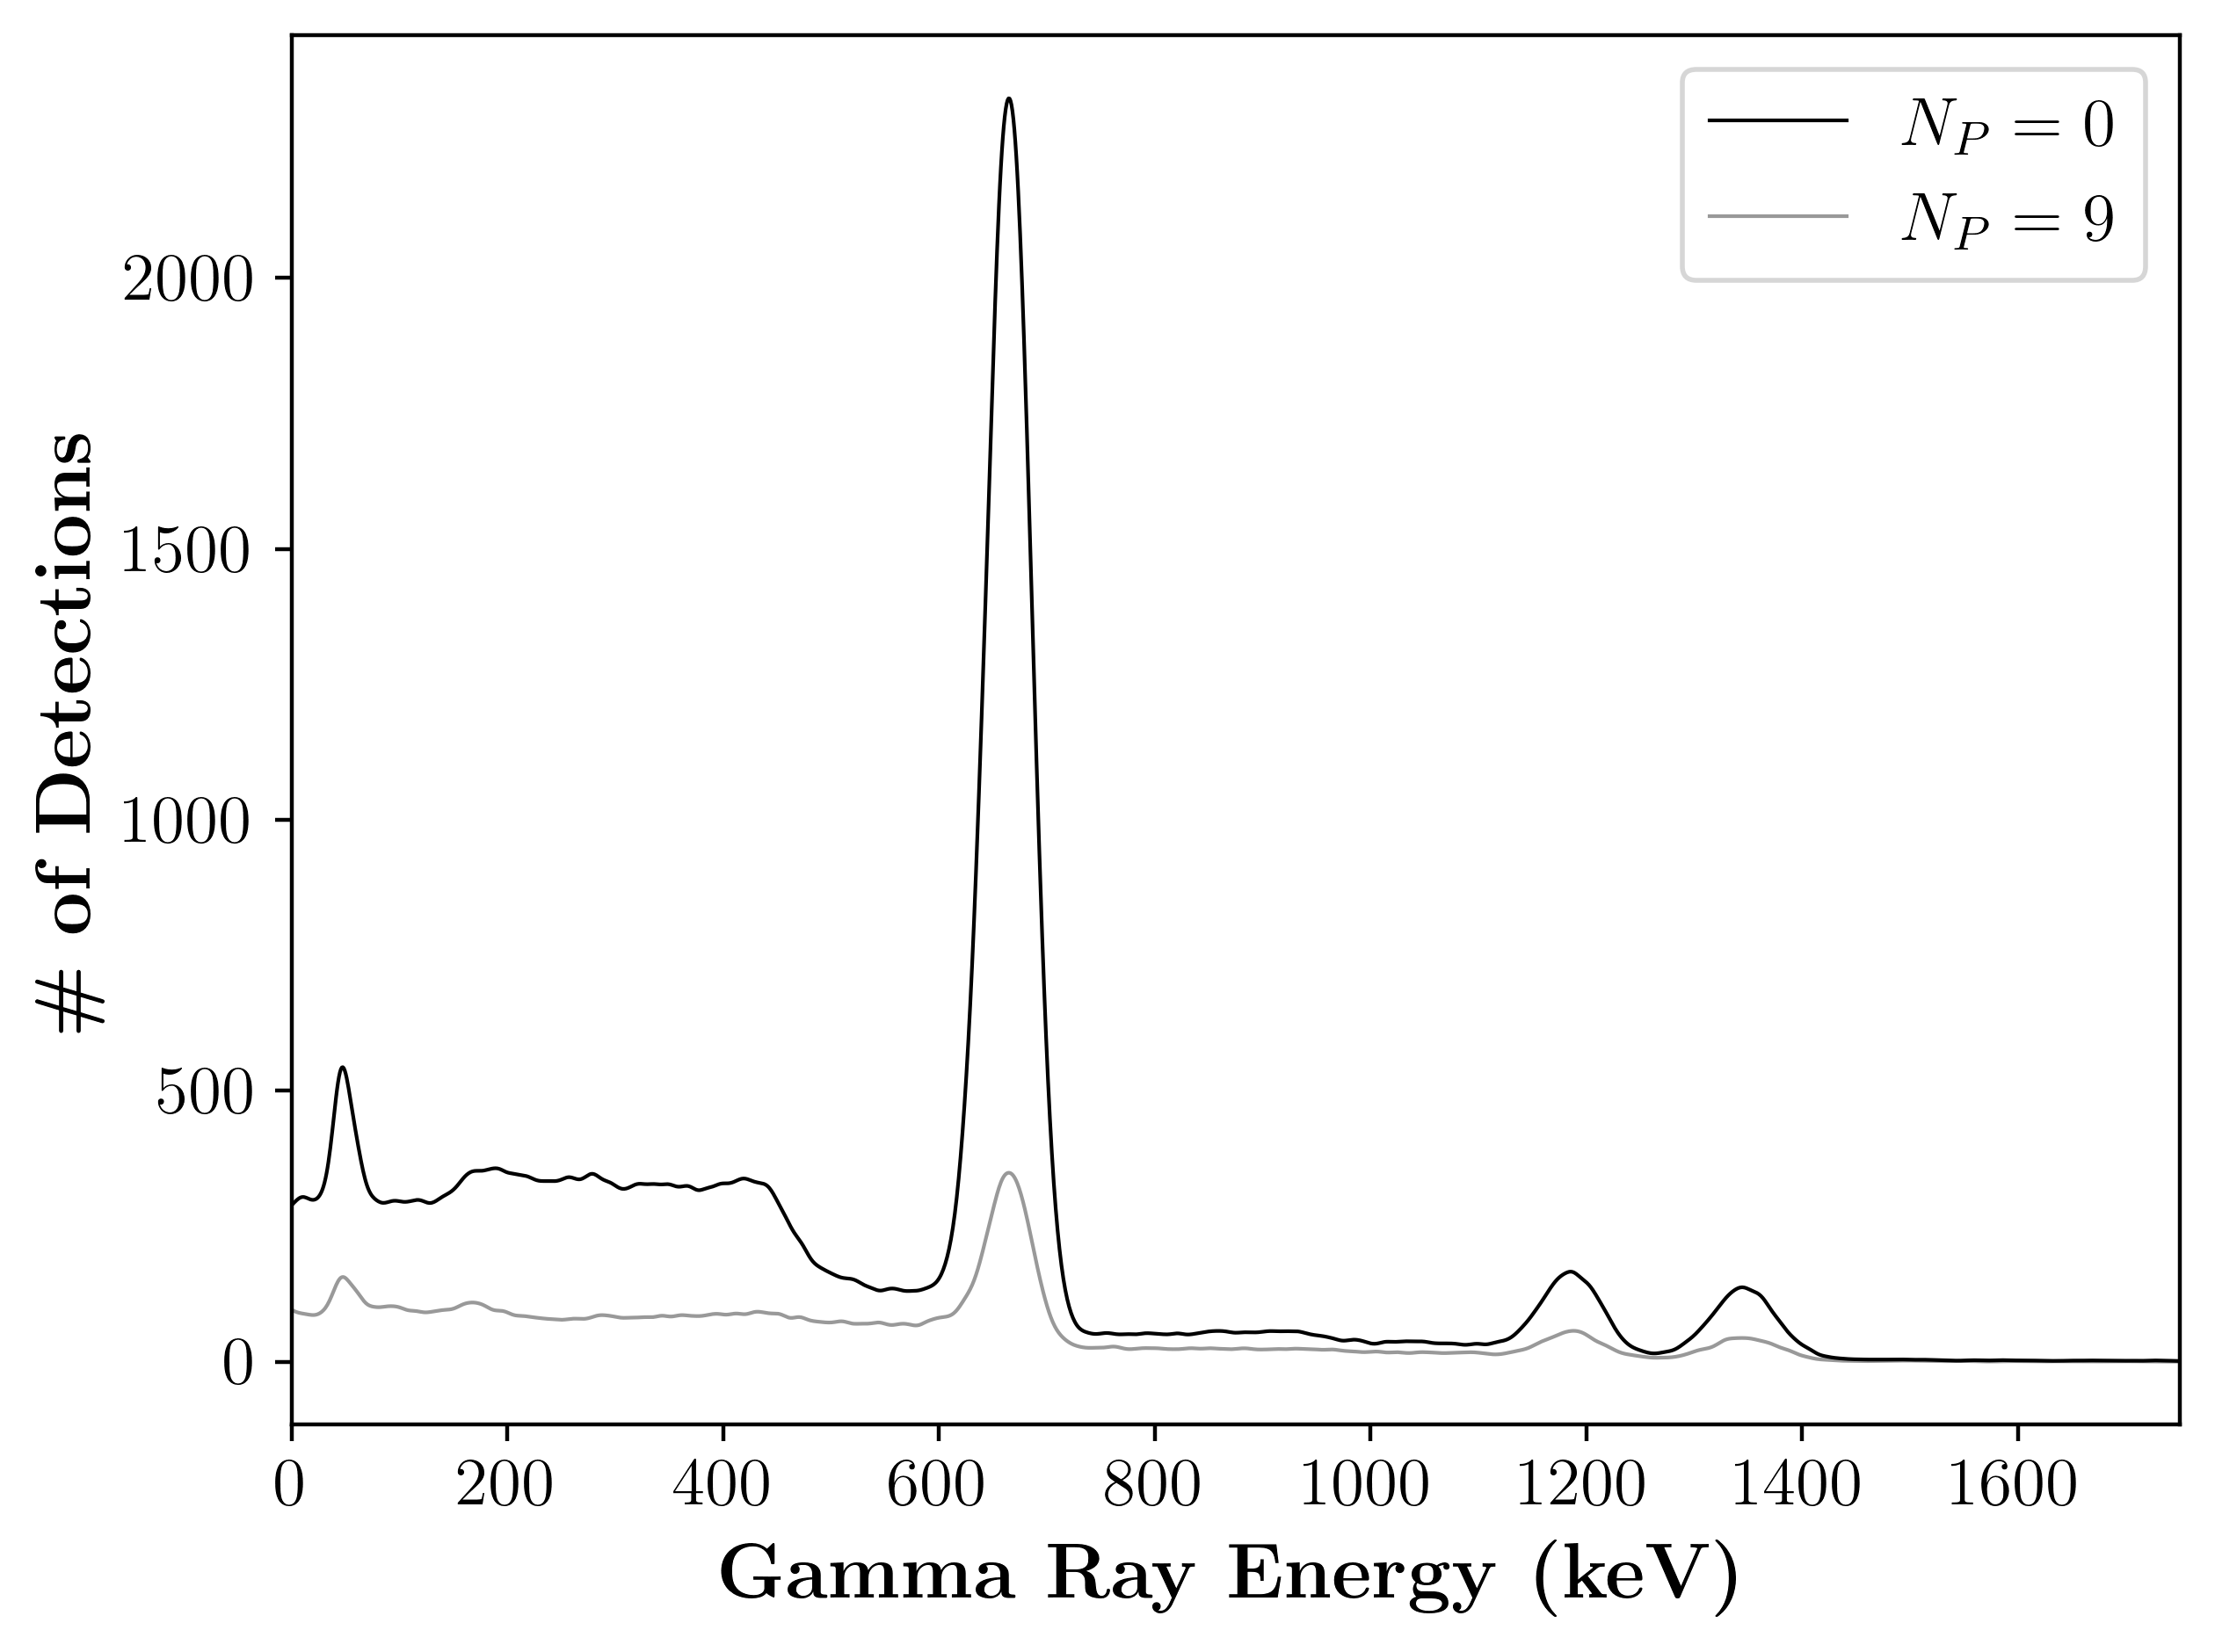
\includegraphics[width=0.75\textwidth]{figures/attenuated_unattenuated_spectra_smooth.png}
    \caption{Spectra comparing the number of counts unattenuated ($N=0$) to the number of counts with 10 attenuator sheets ($N=10$)}
\end{figure}
\begin{figure}[H]
    \centering
    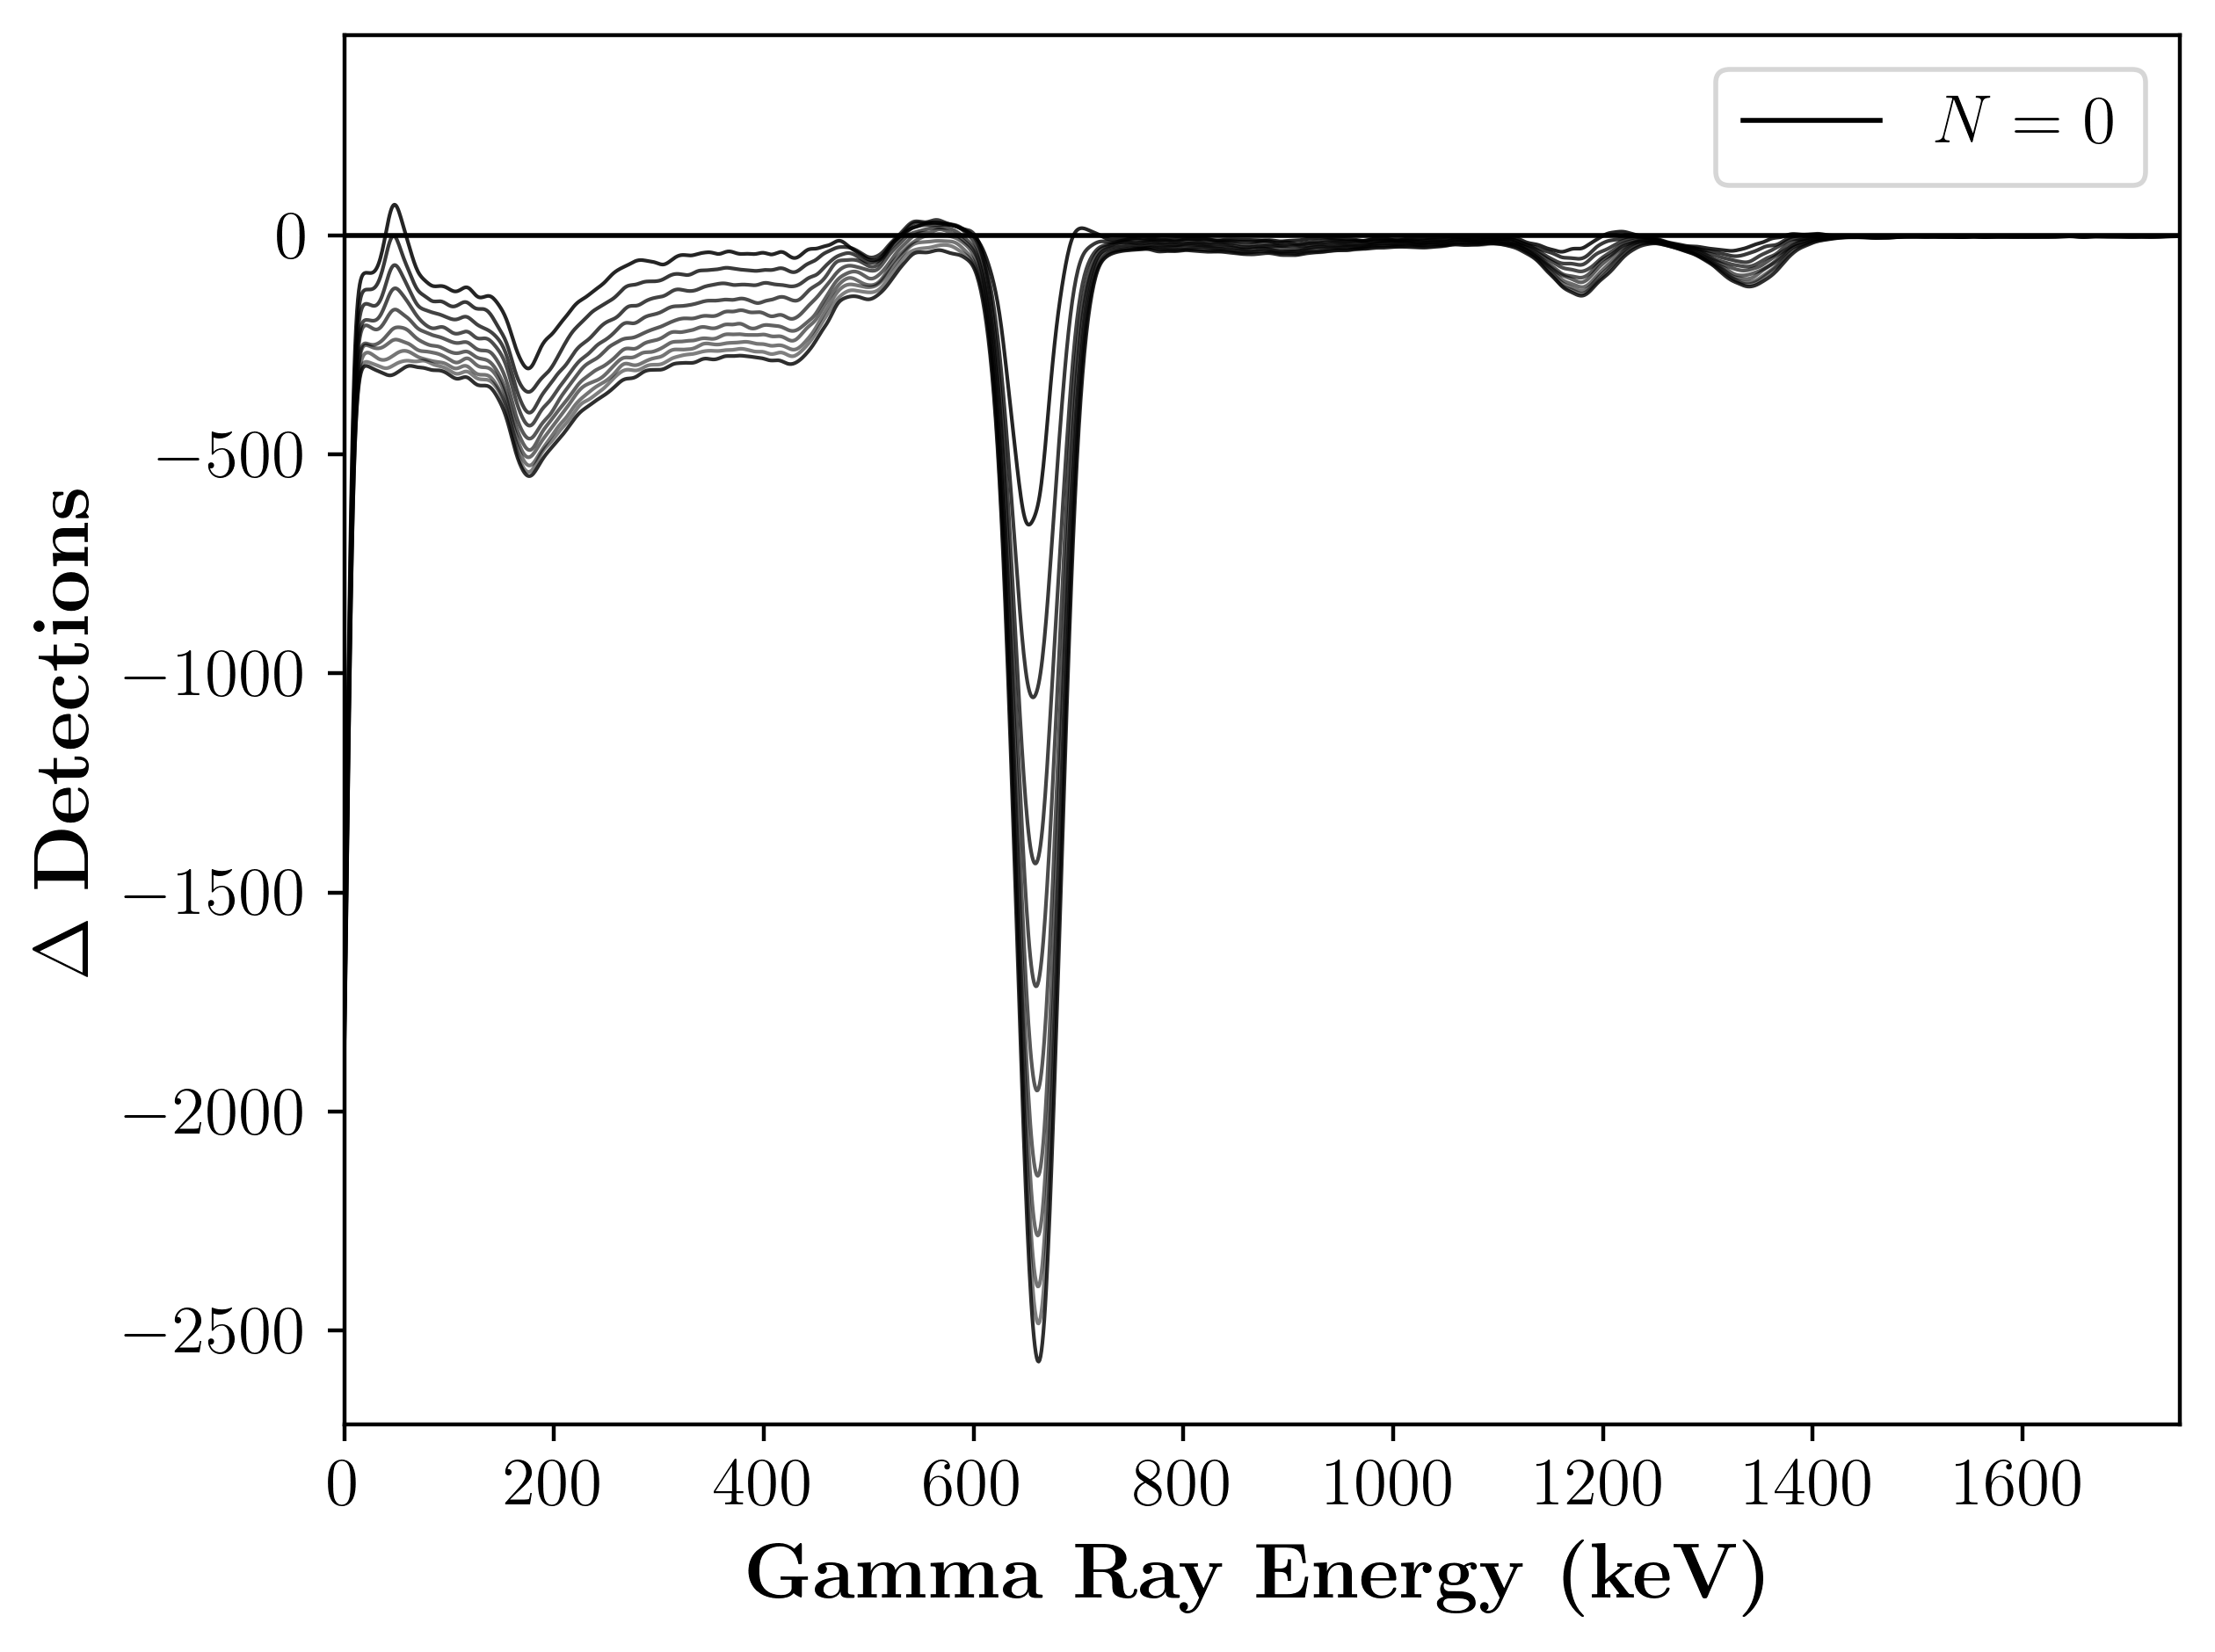
\includegraphics[width=0.75\textwidth]{figures/attenuator_difference_counts_smooth.png}
    \caption{Difference from baseline (no shielding) imparted by $N$ shielding layers present.}
\end{figure}
\section{Aluminum Plate}

\subsection{Recording 1, Plate Present}
\begin{itemize}
    \item sodium cesium 662 keV peak had net area of 130303 $\pm$ 729 net area
    \item cobalt 1274 keV peak had net area of 9087 $\pm$ 315 net area
\end{itemize}
\subsection{Recording 1, Plate Not Present}
\begin{itemize}
    \item sodium cesium 662 keV peak had net area of 147967 $\pm$ 730 net area
    \item cobalt 1274 keV peak had net area of 10251 $\pm$ 329 net area
\end{itemize}
\subsection{Recording 2, Plate Present}
\begin{itemize}
    \item sodium cesium 662 keV peak had net area of 129954 $\pm$ 739 net area
    \item cobalt 1274 keV peak had net area of 8037 $\pm$ 366 net area
\end{itemize}
\subsection{Recording 2, Plate Not Present}
\begin{itemize}
    \item sodium cesium 662 keV peak had net area of 148652 $\pm$ 730 net area
    \item cobalt 1274 keV peak had net area of 10113 $\pm$ 336 net area
\end{itemize}
\subsection{Recording 3, Plate Present}
\begin{itemize}
    \item sodium cesium 662 keV peak had net area of 147154 $\pm$ 741 net area
    \item cobalt 1274 keV peak had net area of 9047 $\pm$ 365 net area
\end{itemize}
\section{Conclusion}
\begin{itemize}
    \item leads HVL thickness would be signifactly thinner than that of aluminum.
    \item 3 layers of lead (approximately) were required to halves the counts, equating to $\approx5.4$mm
    \item comparitevely, 6.31 mm of aluminum only reduced counts by about 15 percent
\end{itemize}
\end{document}